\section{SunSPOT}\label{s:Sunspot}

Die Firma Oracle besitzt im Rahmen seiner Java-Technologie eine Vormachtstellung im Bereich der Smartphones.
Auf der Welt sind schätzungsweise über eine Milliarde Smartphones mit der Java-Technologie lizenziert. Ziel von Oracle ist es, auch in den zukunftsnahen Technologien mit ihrer Programmiersprache Java auszustatten und diese Produkte zu etablieren.\\

Ein erster Schritt in diese Richtung is das von Oracle entwickelte "'SunSPOT"'-Sensornetzwerk. SunSPOT bedeutet "'Sun Small Programmable Object Technology"' und ist eine Plattform für Java-basierte drahtlose Sensornetzwerke. Sie bestätigt den Trend, dass in immer kleiner werdenden Geräten zunehmend leistungsfähigere Technologien eingesetzt werden. Dabei ist wichtig, dass jene Geräte, am Besten drahtlos, miteinander kommunizieren können und jederzeit von überall auf der Welt steuerbar bleiben. Das SunSPOT Starter Paket besteht aus einer Basisstation und 2 Sensoren.\\

\begin{figure}[H] 
	\centering
	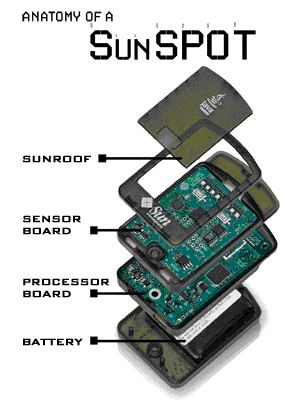
\includegraphics[scale=0.5]{Bilder/spotanatomy.jpg}
	\caption{Anatomie eines Standard SunSPOT-Sensors}
	\label{f:spotaufbau}
\end{figure}

Die Hardware der SunSPOT-Sensoren ist modular aufgebaut. Das bedeutet, dass man die verfügbaren Boards frei nach Belieben aufeinander stecken und somit verbinden kann. Dabei können maximal bis zu 3 Boards + Stromversorgung miteinander verknüpft werden.\\

Das sogenannte eSPOT Prozessor-Board besitzt in der aktuellsten Version eine 400 MHz 32-bit ARM CPU von Atmel, zusammen mit einem Flashspeicher von 8 Megabytes und einem Megabyte SRAM Hauptspeicher. Weiterhin ist es ausgestattet mit einem Radio Transceiver basierend auf IEEE 802.15.4 und einer USB 2.0 - Full Speed Schnittstelle. Der im SunSPOT integrierte Akkumulator hat eine Leistungsfähigkeit von 770mAh. Der maximale Energieverbrauch liegt zwischen 40-100 mA, abhängig von der Nutzung der integrierten LEDs, des Transceivers und anderer angeschlossener Geräte.\\

Der SunSPOT-Sensor wird dazu standardmäßig mit dem eDemo Sensor Board ausgeliefert. Dieses Board besitzt in der aktuellen Version einen 2G/4G/8G 3-Achsen-Beschleunigungssensor, einen Lichtsensor, 8 RGB 24bit LEDs, einen Infrarot-Sender \& Empfänger, ein kleiner Lautsprecher, 2 Knopfschalter, 4 analoge Eingänge, 4 I/O Pins, diverse weitere I$^2$C- und USART-Interfaces, einen EEPROM und 4 100mA Ausgangspins, mit denen es möglich ist, den SunSPOT-Sensor z.b. an weitere Lautsprecher oder andere Geräte anzuschließen.

Weitere Boards, welche man nach Bedarf dazustecken kann, sind das eProto-Board, ein Board welches direkte Zugriffe auf das Prozessorboard ermöglicht und einen SD-Kartenslot besitzt, damit man die Daten dauerhaft speichern kann, das eSerial Board zum Verbinden via RS232 und das eFlash SD-Kartenleser Board.
\cite{d:horan}
\cite{d:spotmain}
\cite{d:spotdemo}
\\

 